\section{Instruzioni all'uso}
Tutte le funzionalità di HDViz sono facilmente reperibili ed nel menu laterale a scomparsa.

\subsection{Caricamento dati}
Inizialmente sono utilizzabili solo le prime voci:
\begin{itemize}
	\item Salva/Carica sessione;
	\item Carica dati dal database;
	\item Carica dati da CSV;
\end{itemize}
Tutte e tre aprono una finestra di dialogo per compiere le operazioni indicate. In particolare:
\begin{itemize}
	\item La finestra per il caricamento dei dati dal database permette di scegliere uno dei dataset presenti nel database ed effettuare immediatamente una selezione delle dimensioni da caricare;
	\item  La finestra per il caricamento dei dati da file CSV permette anche la selezione delle dimensioni che si desidera utilizzare (di default vengono utilizzate tutte quelle caricate)
	\begin{figure}[h]
		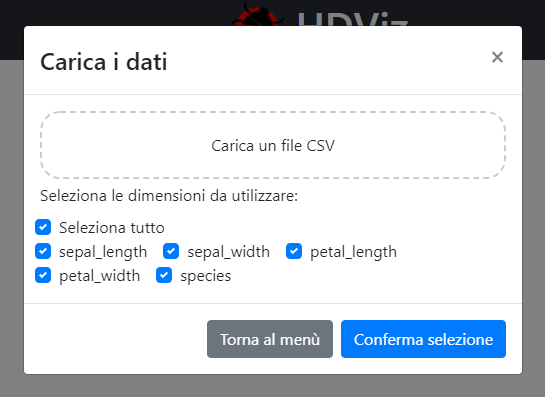
\includegraphics[scale=0.5]{Images/CaricamentoCSV.png}
		\centering
		\caption{Caricamento dati da file CSV}
	\end{figure}
\end{itemize}
   
Una volta caricati i dati è possibile selezionare anche tutte le altre voci del menu. Per la preparzione dei dati sono presenti le seguenti voci:

\begin{itemize}
	\item Riduci dimensioni;
	
	\item Calcola la distanza.
\end{itemize}

\subsection{Riduzion dimensionale} 
Cliccando sulla voce "riduci dimensioni", si apre una finestra che permette di scegliere quali dimensioni utilizzare per la riduzione, quale algoritmo (tra Fastmap, LLE, Isomap e TSNE) e, in base a questa ultima scelta una serie di parametri per eseguire la riduzione come più si preferisce.
\begin{figure}[h]
		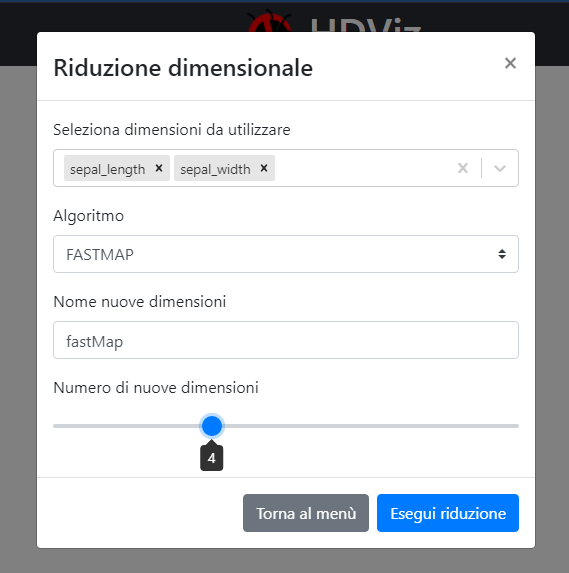
\includegraphics[scale=0.5]{Images/RiduzioneDimensionale.png}
		\centering
		\caption{Finestra per la riduzione dimensionale}
\end{figure}

\subsection{Calcolo della distanza}
Cliccando sulla voce "calcola distanza", si apre una finestra che permette di scegliere quali dimensioni utilizzare per effettuare il calcolo, quale funzione di distanza (tra Euclidea, Camberra, Chebyshev e Manhattan) e il nome da dare alla nuova matrice delle distanze creata.
\begin{figure}[h]
		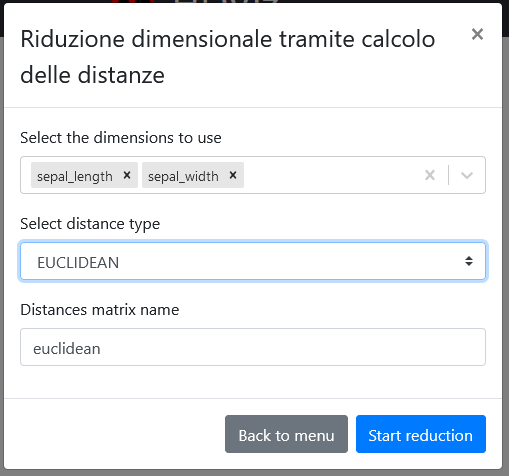
\includegraphics[scale=0.5]{Images/CalcoloDistanze.png}
		\centering
		\caption{Finestra per la riduzione dimensionale tramite il calcolo delle distanze}
\end{figure}

In ogni caso l'applicazione di algoritmi di riduzione dimensionale o funzioni per il calcolo della distanza non sono obbligatori per la visualizzazione dei dati. È infatti possibile, subito dopo aver caricato i dati, scegliere il grafico che più si preferisce tra quelli proposti, ognuno con la sua voce nel menu:

Scatterplot Matrix

Adjency Matrix

Heat Map

Force Field

Linear Projection

Una volta selezionata una di queste si aprirà una form sulla destra attraverso la quale sarà possibile modificare la visualizzazione del grafico, in termini di dimensioni da applicare agli assi, dimensione per l'applicazione del colore sui punti o, per le visualizzazioni che ne fanno uso, è possibile scegliere la matrice delle distanze da utilizzare tra quelle calcolate precedentemente. Da notare come inizialmente tutti i campi siano settati a "No dimension".
Tale form è accompagnata da un bottone per nasconderla e centralizzare il grafico nello schermo per concentrarsi solamente sull'analisi del grafico.